\documentclass[CJK]{beamer}
\usepackage{CJKutf8}
\usepackage{beamerthemesplit}
\usetheme{Malmoe}
\useoutertheme[footline=authortitle]{miniframes}
\usepackage{amsmath}
\usepackage{amssymb}
\usepackage{graphicx}
\usepackage{eufrak}
\usepackage{color}
\usepackage{slashed}
\usepackage{simplewick}
\usepackage{tikz}
\usepackage{tcolorbox}
\graphicspath{{../figures/}}
%%figures
\def\lfig#1#2{\includegraphics[width=#1 in]{#2}}
\def\tfig#1#2{\includegraphics[height=#1 in]{#2}}
\def\addfig#1#2{\begin{center}\includegraphics[width=#1 in]{#2}\end{center}}
\def\wulian{
\includegraphics[width=0.18in]{emoji_wulian.jpg}}
\def\bigwulian{
\includegraphics[width=0.35in]{emoji_wulian.jpg}}
\def\bye{
\includegraphics[width=0.18in]{emoji_bye.jpg}}
\def\bigbye{
\includegraphics[width=0.35in]{emoji_bye.jpg}}
\def\huaixiao{
\includegraphics[width=0.18in]{emoji_huaixiao.jpg}}
\def\bighuaixiao{
\includegraphics[width=0.35in]{emoji_huaixiao.jpg}}
\def\jianxiao{
\includegraphics[width=0.18in]{emoji_jianxiao.jpg}}
\def\bigjianxiao{
\includegraphics[width=0.35in]{emoji_jianxiao.jpg}}
%% colors
\def\blacktext#1{{\color{black}#1}}
\def\bluetext#1{{\color{blue}#1}}
\def\redtext#1{{\color{red}#1}}
\def\darkbluetext#1{{\color[rgb]{0,0.2,0.6}#1}}
\def\skybluetext#1{{\color[rgb]{0.2,0.7,1.}#1}}
\def\cyantext#1{{\color[rgb]{0.,0.5,0.5}#1}}
\def\greentext#1{{\color[rgb]{0,0.7,0.1}#1}}
\def\darkgray{\color[rgb]{0.2,0.2,0.2}}
\def\lightgray{\color[rgb]{0.6,0.6,0.6}}
\def\gray{\color[rgb]{0.4,0.4,0.4}}
\def\blue{\color{blue}}
\def\red{\color{red}}
\def\green{\color{green}}
\def\darkgreen{\color[rgb]{0,0.4,0.1}}
\def\darkblue{\color[rgb]{0,0.2,0.6}}
\def\skyblue{\color[rgb]{0.2,0.7,1.}}
%%control
\def\be{\begin{equation}}
\def\ee{\nonumber\end{equation}}
\def\bea{\begin{eqnarray}}
\def\eea{\nonumber\end{eqnarray}}
\def\bch{\begin{CJK}{UTF8}{gbsn}}
\def\ech{\end{CJK}}
\def\bitem{\begin{itemize}}
\def\eitem{\end{itemize}}
\def\bcenter{\begin{center}}
\def\ecenter{\end{center}}
\def\bex{\begin{minipage}{0.2\textwidth}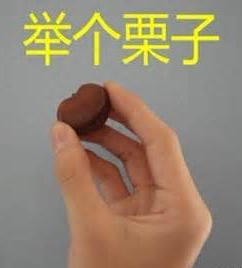
\includegraphics[width=0.6in]{jugelizi.png}\end{minipage}\begin{minipage}{0.76\textwidth}}
\def\eex{\end{minipage}}
\def\chtitle#1{\frametitle{\bch#1\ech}}
\def\bmat#1{\left(\begin{array}{#1}}
\def\emat{\end{array}\right)}
\def\bcase#1{\left\{\begin{array}{#1}}
\def\ecase{\end{array}\right.}
\def\bmini#1{\begin{minipage}{#1\textwidth}}
\def\emini{\end{minipage}}
\def\tbox#1{\begin{tcolorbox}#1\end{tcolorbox}}
\def\pfrac#1#2#3{\left(\frac{\partial #1}{\partial #2}\right)_{#3}}
%%symbols
\def\newt#1#2{\left(\begin{array}{c}#1\\ #2\end{array}\right)}
\def\reof#1{\,\mathrm{Re}{\left(#1\right)\,}}
\def\imof#1{\,\mathrm{Im}{\left(#1\right)\,}}
\def\Arg#1{\,\mathrm{Arg}\,#1\,}
\def\bropt{\,(\ \ \ )}
\def\sone{$\star$}
\def\stwo{$\star\star$}
\def\sthree{$\star\star\star$}
\def\sfour{$\star\star\star\star$}
\def\sfive{$\star\star\star\star\star$}
\def\rint{{\int_\leftrightarrow}}
\def\roint{{\oint_\leftrightarrow}}
\def\stdHf{{\textit{\r H}_f}}
\def\deltaH{{\Delta \textit{\r H}}}
\def\ii{{\dot{\imath}}}
\def\skipline{{\vskip0.1in}}
\def\skiplines{{\vskip0.2in}}
\def\lagr{{\mathcal{L}}}
\def\hamil{{\mathcal{H}}}
\def\vecv{{\mathbf{v}}}
\def\vecx{{\mathbf{x}}}
\def\vecy{{\mathbf{y}}}
\def\veck{{\mathbf{k}}}
\def\vecp{{\mathbf{p}}}
\def\vecn{{\mathbf{n}}}
\def\vecA{{\mathbf{A}}}
\def\vecP{{\mathbf{P}}}
\def\vecsigma{{\mathbf{\sigma}}}
\def\hatJn{{\hat{J_\vecn}}}
\def\hatJx{{\hat{J_x}}}
\def\hatJy{{\hat{J_y}}}
\def\hatJz{{\hat{J_z}}}
\def\hatj#1{\hat{J_{#1}}}
\def\hatphi{{\hat{\phi}}}
\def\hatq{{\hat{q}}}
\def\hatpi{{\hat{\pi}}}
\def\vel{\upsilon}
\def\Dint{{\mathcal{D}}}
\def\adag{{\hat{a}^\dagger}}
\def\bdag{{\hat{b}^\dagger}}
\def\cdag{{\hat{c}^\dagger}}
\def\ddag{{\hat{d}^\dagger}}
\def\hata{{\hat{a}}}
\def\hatb{{\hat{b}}}
\def\hatc{{\hat{c}}}
\def\hatd{{\hat{d}}}
\def\hatN{{\hat{N}}}
\def\hatH{{\hat{H}}}
\def\hatp{{\hat{p}}}
\def\Fup{{F^{\mu\nu}}}
\def\Fdown{{F_{\mu\nu}}}
\def\newl{\nonumber \\}
\def\vece{\mathrm{e}}
\def\calM{{\mathcal{M}}}
\def\calT{{\mathcal{T}}}
\def\calR{{\mathcal{R}}}
\def\barpsi{\bar{\psi}}
\def\baru{\bar{u}}
\def\barv{\bar{\upsilon}}
\def\qeq{\stackrel{?}{=}}
\def\torder#1{\mathcal{T}\left(#1\right)}
\def\rorder#1{\mathcal{R}\left(#1\right)}
\def\contr#1#2{\contraction{}{#1}{}{#2}#1#2}
\def\trof#1{\mathrm{Tr}\left(#1\right)}
\def\trace{\mathrm{Tr}}
\def\comm#1{\ \ \ \left(\mathrm{used}\ #1\right)}
\def\tcomm#1{\ \ \ (\text{#1})}
\def\slp{\slashed{p}}
\def\slk{\slashed{k}}
\def\calp{{\mathfrak{p}}}
\def\veccalp{\mathbf{\mathfrak{p}}}
\def\Tthree{T_{\tiny \textcircled{3}}}
\def\pthree{p_{\tiny \textcircled{3}}}
\def\dbar{{\,\mathchar'26\mkern-12mu d}}
\def\erf{\mathrm{erf}}
\def\const{\mathrm{constant}}
\def\pheat{\pfrac p{\ln T}V}
\def\vheat{\pfrac V{\ln T}p}
%%units
\def\fdeg{{^\circ \mathrm{F}}}
\def\cdeg{^\circ \mathrm{C}}
\def\atm{\,\mathrm{atm}}
\def\angstrom{\,\text{\AA}}
\def\SIL{\,\mathrm{L}}
\def\SIkm{\,\mathrm{km}}
\def\SIyr{\,\mathrm{yr}}
\def\SIGyr{\,\mathrm{Gyr}}
\def\SIV{\,\mathrm{V}}
\def\SImV{\,\mathrm{mV}}
\def\SIeV{\,\mathrm{eV}}
\def\SIkeV{\,\mathrm{keV}}
\def\SIMeV{\,\mathrm{MeV}}
\def\SIGeV{\,\mathrm{GeV}}
\def\SIcal{\,\mathrm{cal}}
\def\SIkcal{\,\mathrm{kcal}}
\def\SImol{\,\mathrm{mol}}
\def\SIN{\,\mathrm{N}}
\def\SIHz{\,\mathrm{Hz}}
\def\SIm{\,\mathrm{m}}
\def\SIcm{\,\mathrm{cm}}
\def\SIfm{\,\mathrm{fm}}
\def\SImm{\,\mathrm{mm}}
\def\SInm{\,\mathrm{nm}}
\def\SImum{\,\mathrm{\mu m}}
\def\SIJ{\,\mathrm{J}}
\def\SIW{\,\mathrm{W}}
\def\SIkJ{\,\mathrm{kJ}}
\def\SIs{\,\mathrm{s}}
\def\SIkg{\,\mathrm{kg}}
\def\SIg{\,\mathrm{g}}
\def\SIK{\,\mathrm{K}}
\def\SImmHg{\,\mathrm{mmHg}}
\def\SIPa{\,\mathrm{Pa}}
%page
\def\secpage#1#2{\begin{frame}\bch\bcenter{\bf \Huge #1} \skipline \tbox{#2}\ecenter\ech\end{frame}}

\def\courseurl{https://github.com/zqhuang/SYSU\_TD}

\def\tpage#1#2{
\begin{frame}
\begin{center}
\begin{Large}
\bch
热学 \\
第#1讲 #2

{\vskip 0.3in}

黄志琦

\ech
\end{Large}
\end{center}

\vskip 0.2in

\bch
教材:《热学》第二版,赵凯华,罗蔚茵,高等教育出版社
\ech

\bch
课件下载
\ech
\courseurl
\end{frame}
}

\def\bfr#1{
\begin{frame}
\chtitle{#1} 
\bch
}

\def\efr{
\ech 
\end{frame}
}

  \date{}
  \begin{document}
  \bch
\tpage{27}{哈密顿量和蛙跳法}

\begin{frame}
\frametitle{本讲内容}
\tableofcontents
\end{frame}

\section{Review and Practices}

\begin{frame}
  \frametitle{看看多少人已经下车了}

  \addfig{0.7}{think1.jpg}
  
  一个半径为 $R$ 的实心均匀球,现在调控球面上的温度为:
$$T(r,\theta,\phi)|_{r=R} = T_0+T_1\,\mathrm{Re}\left[Y_{7,4}(\theta,\phi)\right].$$
其中 $\mathrm{Re}$表示取实部,$r,\theta,\phi$ 是以球心为原点建立的球坐标系, $T_0,T_1$ 为常量。

则球内部的温度 $T(r, \theta,\phi)$ ($r < R$) 是怎样的?
\end{frame}



\begin{frame}
  \frametitle{看看多少人已经下车了}
  \addfig{0.7}{think2.jpg}

  大致估算
  $$\int_{10!}^{1000!}\left[N_{100}(x)\right]^2 dx $$
  的值。
  
\end{frame}

\begin{frame}
  \frametitle{看看多少人已经下车了}
  \addfig{0.4}{think0.jpg}
  
  如果 $\hat{A}$ 是算符,定义
  $$ e^{\hat{A}} = \sum_{n=0}^\infty \frac{1}{n!}\hat{A}^n.$$

  那么,如果有两个算符 $\hat{A},\hat{B}$,
  $$ e^{\hat{A}+\hat{B}} =  e^{\hat{A}}  e^{\hat{B}}$$
  一般还成立吗?如果已知这两个算符对易呢?
  
  
\end{frame}


\section{Leapfrog Method}

\begin{frame}
  \frametitle{哈密顿方程}
  设 $q$ 为广义坐标, $p$为广义动量。
  
  如果已知哈密顿量 $H(p, q)$, 则$(x,p)$ 的时间导数由哈密顿方程给出:

  $$\dot p = -\frac{\partial H}{\partial q}$$    
  $$\dot q = \frac{\partial H}{\partial p}$$

\end{frame}


\begin{frame}
  \frametitle{练练手,熟悉一下}

  \addfig{0.7}{think2.jpg}
  
  设 $H = \frac{1}{2}p^2$,写出哈密顿方程。

\end{frame}


\begin{frame}
  \frametitle{练练手,熟悉一下}

  \addfig{0.7}{think3.jpg}
  
  设 $H = \frac{1}{2}q^2$,写出哈密顿方程。

\end{frame}

\begin{frame}
  \frametitle{ 烧脑的观点来了}
  我们可以把任意二元函数 $H(\cdot, \cdot)$等价地看成一个 $(p, q)$ 到 $(\dot p, \dot q)$ 的映射规则:
  
  $$\dot p = -\frac{\partial H(p,q)}{\partial q}$$
  $$\dot q = \frac{\partial H(p,q)}{\partial p}$$

  抽象地写就是

  $$\begin{pmatrix}
    \dot p \\
    \dot q
  \end{pmatrix}
  = \hat{H} \begin{pmatrix}
     p \\
     q
  \end{pmatrix}
  $$
  这里的 $\hat{H}$ 就是一个“操作规则”, 或者说,一个算符。这个算符把函数 $(p, q)$映射为了函数 $(\dot p, \dot q)$。注意一般来说这个算符是非线性的。
  
\end{frame}

\begin{frame}
  \frametitle{抽象解}
  虽然 $\hat{H}$ 这个算符一般是非线性的,已经复杂到无法用矩阵来描述了,但这不妨碍我们抽象地把

  $$\begin{pmatrix}
    \dot p \\
    \dot q
  \end{pmatrix}
  = \hat{H} \begin{pmatrix}
     p \\
     q
  \end{pmatrix}  $$
  
  进行“积分”,得到
  
  $$\begin{pmatrix}
    p(t) \\
    q(t)
  \end{pmatrix}
  = e^{\hat{H}t} \begin{pmatrix}
     p(0) \\
     q(0)
  \end{pmatrix}  $$

  这里的
  $$e^{\hat{H}t}:=\sum_{n=0}^\infty \frac{1}{n!}\hat{H}^nt^n.$$  
\end{frame}

\begin{frame}
  \frametitle{例子:谐振子}
  一维谐振子的哈密顿量可以写成:
  $$ H(p, q) =   \frac{1}{2} p^2 + \frac{1}{2} q^2$$
  其中 $q$ 是位移,$p$ 是动量。
  
  (请自行根据量纲补充合适的单位,这些不是我们讨论的重点)
\end{frame}


\begin{frame}
  \frametitle{例子:谐振子}
  哈密顿方程为:
  $$\dot p = -q $$
  $$\dot q = p $$

  简单起见,假设初始条件为  $p(0)= 0$, $q(0)=1$。我们想求出以后的 $p(t), q(t)$是如何演化的。

  \skipline
  
  假装我们的高数已经下车,但是C语言刚刚上车。准备用数值方法求解这个问题。

  \skipline
  

  (我其实主要是针对对没有解析解的情况,只是为了说明问题方便而用你们熟悉的谐振子作为例子)  
\end{frame}


\begin{frame}
  \frametitle{C语言来了}

  int N = 10000;
  
  double dt = 0.01,  p = 0, q = 1;

  for(int i = 0; i $<$ N; i++)\{
    
  \  p = p - q * dt;

  \  q = q + p * dt;
  
  \}

  printf("\%f \%f  \%f$\backslash$n", N*dt, p, q);

  \skiplines
  
  实测输出结果:

  100.000000 0.506013  0.865060
  
\end{frame}


\begin{frame}
  \frametitle{稍稍换一下次序}

  int N = 10000;
  
  double dt = 0.01,  p = 0, q = 1;

  for(int i = 0; i $<$ N; i++)\{    

  \  q = q + p * dt;

  \  p = p - q * dt;  
  
  \}

  printf("\%f \%f  \%f$\backslash$n", N*dt, p, q);

  \skiplines

  实测输出结果:

  100.000000 0.506013  0.860000
  
\end{frame}


\begin{frame}

  \addfig{0.7}{think.jpg}

  前面两段代码为何会给出不同的结果?
  
\end{frame}


\begin{frame}

  \frametitle{蛙跳法}

  跟严格解 $p(100) = -\sin 100 = 0.5063656$, $q(100) = \cos(100)= 0.86231887$ 做比较,我们发现结果还算是相当不错的。

  \skiplines
  
  这种用哈密顿方程交替更新 $p,q$ 的方法叫做“蛙跳法” (leapfrog method)。它通常能够用很低的内存消耗和算法复杂度给出较好近似结果。

\end{frame}


\begin{frame}
  \frametitle{思考题}

  \addfig{0.7}{think1.jpg}
  
  用级数展开大法证明:
  $$ e^{(\hat{H}_1+\hat{H}_2) \Delta t} \approx e^{\frac{\hat{H}_1\Delta t}{2}} e^{\hat{H}_2\Delta t}  e^{\frac{\hat{H}_1\Delta t}{2}} $$
  误差至多是 $O(\Delta t^3)$ 的量级。

  (推导时要注意 $\hat{H}_1, \hat{H}_2$ 一般是不对易的,即 $\hat{H}_1\hat{H}_2\ne \hat{H}_2\hat{H}_1$)
\end{frame}

\begin{frame}
  \frametitle{蛙跳法的原理}

  \addfig{0.7}{think2.jpg}
  
  把谐振子的哈密顿量拆成两部分的和 $H=H_1+H_2$,其中 $H_1=\frac{1}{2}p^2$, $H_2=\frac{1}{2}q^2$。然后利用前面的近似
  $$ e^{(\hat{H}_1+\hat{H}_2) \Delta t} \approx e^{\frac{\hat{H}_1\Delta t}{2}} e^{\hat{H}_2\Delta t}  e^{\frac{\hat{H}_1\Delta t}{2}} $$
  求解谐振子的 $(p,q)$ 的演化。

  \skiplines
  
  如果取 $H_2=\frac{1}{2}p^2$, $H_1=\frac{1}{2}q^2$,结果会怎样?

  \skiplines
  
  (注意:用$H_1$和 $H_2$单独作为哈密顿量时,程序其实在进行严格求解。也就是误差完全来自于上述算符等式的 $O(\Delta t^3)$误差。)
\end{frame}

\begin{frame}
  \frametitle{蛙跳法的原理}
  当你把很多步连起来的时候,
  $$ e^{(\hat{H}_1+\hat{H}_2) \Delta t} e^{(\hat{H}_1+\hat{H}_2) \Delta t}e^{(\hat{H}_1+\hat{H}_2) \Delta t}\ldots \approx e^{\frac{\hat{H}_1\Delta t}{2}} e^{\hat{H}_2\Delta t}  e^{\hat{H}_1\Delta t} e^{\hat{H}_2\Delta t} e^{\hat{H}_1\Delta t} \ldots $$

  这就是数值计算中的蛙跳法。
  
\end{frame}

\begin{frame}
  \frametitle{思考题}

  \addfig{0.7}{think1.jpg}

  你能把前面的程序加以简单改进,使得在几乎完全相同的计算量下,结果的精度得以大大改善吗?
  
\end{frame}

\begin{frame}
  \frametitle{最后:请欣赏下6阶3重蛙跳}
{\small    
\begin{eqnarray}
e^{(\hat{A}+\hat{B}+\hat{C})dt} &=& e^{c_3\hat{A}dt/2}e^{c_3\hat{B}dt/2}e^{c_3\hat{C}dt}e^{c_3\hat{B}dt/2}e^{(c_3+c_2)\hat{A}dt/2}\nonumber \\
&& \times \, e^{c_2\hat{B}dt/2}e^{c_2\hat{C}dt}e^{c_2\hat{B}dt/2}e^{(c_2+c_1)\hat{A}dt/2} \nonumber \\
&& \times \, e^{c_1\hat{B}dt/2}e^{c_1\hat{C}dt}e^{c_1\hat{B}dt/2}e^{(c_1+c_0)\hat{A}dt/2} \nonumber \\
&& \times \, e^{c_0\hat{B}dt/2}e^{c_0\hat{C}dt}e^{c_0\hat{B}dt/2}e^{(c_0+c_1)\hat{A}dt/2} \nonumber \\
&& \times \, e^{c_1\hat{B}dt/2}e^{c_1\hat{C}dt}e^{c_1\hat{B}dt/2}e^{(c_1+c_2)\hat{A}dt/2} \nonumber \\
&& \times \, e^{c_2\hat{B}dt/2}e^{c_2\hat{C}dt}e^{c_2\hat{B}dt/2}e^{(c_2+c_3)\hat{A}dt/2} \nonumber \\
&& \times \, e^{c_3\hat{B}dt/2}e^{c_3\hat{C}dt}e^{c_3\hat{B}dt/2}e^{c_3\hat{A}dt/2} \nonumber \\
&& + O(dt^7)\ , \nonumber
\end{eqnarray}
\begin{eqnarray}
c_1 &=& -1.17767998417887\ldots \ ,\nonumber \\
c_2 &=& 0.235573213359357\ldots \ ,\nonumber \\
c_3 &=& 0.784513610477560\ldots \ ,\nonumber \\
c_0 &=& 1-2(c_1+c_2+c_3) \ . \nonumber
\end{eqnarray}
}
\end{frame}


\ech
\end{document}
